\chapter{DATA}
\label{ch:data}

The data used to test the hypothesis and aims introduced in the previous chapter are drawn from a set of simulated rs-fMRI sequences and three clinical groups. In this chapter, we will first discuss the need for simulated sequences and the processes used to generate them for our work. Then, we will discuss the clinical images which were taken from several prospective studies of congenital heart defects in three age groups of pediatric patients. These groups were chosen because congenital heart disease (CHD) affects patients throughout their lifespans, and different characteristics in motion patterns have been observed in patients of different ages with and without CHD.

\section{Simulated Sequences} 

There are two major barriers in research surrounding motion correction in rs-fMRIs: gathering data and measuring the effects of the technique. 

The challenge of gathering significant amounts of data is common across the medical domain. Simulating realistic patient scans can mitigate this challenge and make rs-fMRI research more accessible. 

Research on motion correction in rs-fMRIs often focuses on the amount of the positional effects of motion removed from the image. This silver standard is used because the gold standard, the amount of brain signal recovered by motion correction is unknown in clinical images. When an rs-fMRI is simulated, the amount of brain signal in the sequence can be manually specified. The known brain signal can be used to evaluate motion correction techniques with respect to the amount of brain signal recovered by the technique.

In this section, we elaborate on a simulation we designed and implemented to address both of these barriers.

\subsection{Background}

It is difficult to obtain enough data from a large number of subjects to perform large-scale studies in the medical domain. Collaborators can band together to create a larger and more diverse data set by participating in multicenter studies, though there are some challenges associated with multicenter studies. Each site will have a different scanner, potentially with different field strengths and from different manufacturers. Even ignoring the challenges of harmonizing data obtained using scanners from different companies, each scanner has its own set of unique inhomogeneities in the primary magnetic field. Additional scans of inanimate or human phantoms may be necessary to characterize the differences between all of the scanners involved in a multicenter study.

The second barrier to motion correction in rs-fMRI research is the complexity of identifying a gold standard metric to use when evaluating motion correction techniques. The current criteria for determining the usability of an rs-fMRI sequence developed by Power et al. evaluate motion correction techniques in terms of the reduction of positional differences and signal differences between neighboring volumes. Unfortunately, this approach does not measure the amount of signal recovered or lost through motion correction. A true gold standard evaluation of motion correction would be able to evaluate the BOLD signal present in the image before and after correction. If the BOLD signal prior to the patient motion was known, though, there would be no need for image processing in the first place: we would already have the data we are trying to obtain with motion correction.

We address these two barriers by creating a mechanism for generating simulated image sequences. The generated sequences contain simulated brain signal based in areas of the brain associated with resting-state connectivity, scanner noise, and patient motion. Our mechanism can create large quantities of unique image sequences. The simulated image sequences can also serve as a gold standard for evaluating volume registration and motion correction techniques: the signals and noise sources added to the sequence are known because they are generated as part of the simulation.

\subsection{SPECTr: Simulated Phantom Emulating Cranial Transformations}

Our mechanism is called Simulated Phantom Emulating Cranial Transformations (SPECTr). A phantom is an object designed to have material properties that mimic those of a specific tissue type or organ. Phantoms, either manufactured objects or healthy humans, are used in multicenter studies to obtain images of the same object or person from multiple scanners. These images are used to harmonize the data taken from different sites. We call our simulated sequence a phantom because the baseline image itself is known as are the signals added to it to simulate brain activity. 

When developing the pipeline for SPECTr, it was important to consider the multiple facets of rs-fMRI sequences. The BOLD signal must be present in areas of the brain associated with resting-state neuronal networks. The effects of motion and various impacts they have on the BOLD signal must also be present. As discussed in Chapter \ref{ch:mri}, the three effects of motion are positional, spin history, and susceptibility. The positional effects of motion are straightforward to implement. For simplicity, we model the spin history and susceptibility effects as a single source of in-scanner noise. 

\subsection{Materials}

In order to simulate the resting-state BOLD signal in an fMRI, two pieces of anatomical information are required. The first is structural information about the brain. The second is the location of functional networks associated with the resting-state BOLD signal.

While it is possible to use clinical images for the structural information, the goal of SPECTr is to be generalizable both for our use and for the use of other researchers. Additionally, clinical images inherently contain some degree of signal from some neuronal processes which could obfuscate the simulated BOLD signal. 

In 1992, the International Consortium for Brain Mapping was formed to develop a set of standards for what is considered a healthy human brain. They used their criteria to develop an initial set of ``average'' brain structural scans based on scans from healthy volunteers. This original set of average brain scans incorporates scans from 305 subjects and is referred to as the MNI305 data. As MRI technology has evolved, the spatial resolution capabilities of the MRI scanners have increased. In 2001, another set of 152 healthy volunteers was recruited to create a higher resolution data set. The scans from the new cohort were linearly registered to the MNI305 data to create the new MNI152 images. % ELEPHANTS citations needed

Herein, we use the MNI152 data set as available at the website for the McConnell Brain Imaging Centre at McGill University \cite{Fonov2009} \cite{Fonov2011}. This data set contains five images: a T1-weighted scan, a T2-weighted scan, a proton density-weighted scan, and two binary masks for the head and the brain. Each of the structural scans was designed to highlight the properties of different tissues in and around the brain. Proton density scans were developed for the purpose of detecting the blood-related signal. As BOLD images essentially perform the same purpose as a proton density image over a period of minutes, we choose to use the proton density-weighted scan as the structural base for the simulated images. 

The functional network information is more difficult to find than structural atlases. The Functional Imaging in Neuropsychiatric Disorders Lab at Stanford has developed two sets of functional atlases. The atlases are divided into regions of interest (ROIs) associated with individual networks. The first set of atlases contains 90 functional ROIs which compose 14 networks \cite{Shirer2012}. The second set of atlases contains 499 functional ROIs and has more gray matter coverage \cite{Altmann2015}. We chose to use the original ROIs associated with the dorsal and ventral default mode networks.

\subsection{Simulation Pipeline}

\subsubsection{Baseline Sequence}

\begin{figure}
\centering

\includegraphics[width=.6\textwidth]{5/pipeline.png}
\caption{An overview of the SPECTr simulation pipeline. Using atlas data, a simulated phantom containing brain signal, scanner noise, and patient motion is generated.}
\label{ch5:spectr_flow}
\end{figure}

The process for generating a simulated sequence using the data discussed in the previous section has several steps. An overview of the pipeline can be seen in Figure \ref{ch5:spectr_flow} We cover these steps in detail in this section.

The MNI152 proton density image is a whole head image. To remove the skull, we apply the brain mask to the proton density-weighted image. The resulting image contains only brain tissue.

The spatial resolution of the structural brain image is 1 mm$^3$, but the spatial resolution for a single volume in an rs-fMRI sequence is less granular at 4mm$^3$. In order to achieve this resolution, the structural volume must be downsampled. After the downsampling, the size of the structural image is reduced from 181x217x181 voxels to 45x54x45 voxels. 

Now that the structural image is the correct spatial resolution, it must be replicated to create the temporal sequence. Part of this step includes creating a new dimension in the data. The affine matrix which represents the resolution of the image has the following structure:

\begin{equation}
\begin{bmatrix}
 r_x &  0   &  0   & c_x\\ 
 0   &  r_y &  0   & c_y \\ 
 0   &  0   &  r_z & c_z \\ 
 0   &  0   &  0   & 1 
\end{bmatrix}
\end{equation}

\noindent where $r_x, r_y,$ and $r_z$ represent the spatial resolution in the $x, y,$ and $z$ axes, respectively and $c_x, c_y,$ and $c_z$ represent the location of the origin in voxels. To convert the image from a 3D volume to a 4D sequence, we add a row and a column to this matrix so that it now has the structure:

\begin{equation}
\begin{bmatrix}
 r_x &  0   &  0   & 0 & c_x\\ 
 0   &  r_y &  0   & 0 & c_y \\ 
 0   &  0   &  r_z & 0 & c_z \\ 
 0   &  0   &  0   & t & 0 \\
 0   &  0   &  0   & 0 & 1 
\end{bmatrix}
\end{equation}

\noindent where $t$ is the desired temporal resolution. We choose a temporal resolution of 2 seconds for our simulated sequence. The downsampled image volume is replicated and concatenated along the new temporal dimension to create a sequence that is 150 image volumes long. This sequence is referred to as the base phantom sequence as it contains no brain signal, noise, or motion.

\subsubsection{Brain Signal}

The next step in the pipeline is to add the BOLD signal to the sequence. 
We combine the functional ROIs from the dorsal and ventral default mode networks into a single binary functional ROI image. This image is referred to as the default mode network (DMN) mask. 

For each nonzero voxel in the DMN mask, a temporal signal is generated. We chose to model the BOLD response as a cosine signal following the formula:

\begin{equation}
s(\vec{v}, t) = a*(cos(f_0 * (t-t_{shift})) - a_shift).
\label{ch5:bold_eq}
\end{equation}

\noindent This equation is for a scaled cosine function with both temporal and amplitude shifts. The temporal and amplitude shifts, $t_{shift}$ and $a_{shift}$ respectively, are randomly generated for each voxel from uniform distributions. Once chosen, they are consistent across the voxel's generated temporal signal. The other parameters, $a$ and $f_0$, were specified using existing research. 

In 2007, Biswal et al. performed a study evaluating methods to reduce changes in the BOLD signal not directly related to brain activity (i.e., vascularity). They identified a low-frequency spectral amplitude of 0.04 Hz as the highest frequency related to the BOLD signal consistent not only through scans of individual patients but in group-wise analyses. Based on their work, we chose the fundamental frequency of $f_0$ to be 0.04 Hz \cite{Biswal2007}. 

The scaling factor $a$ was chosen based on Power et al.'s usability criteria. As they state that any signal change between volumes above 2.5\% of the maximum voxel value is unlikely to be due to brain activity, we used an amplitude of 20 units on a scaled voxel value range of [0, 1000] \cite{Power2012}. 

The generated BOLD signals were added to the baseline image sequence but were also saved in a separate image sequence file for reference during analysis. The generated sequence with only the BOLD signal is referred to as the brain signal sequence.

\subsubsection{Scanner Noise}

\begin{figure}
\centering
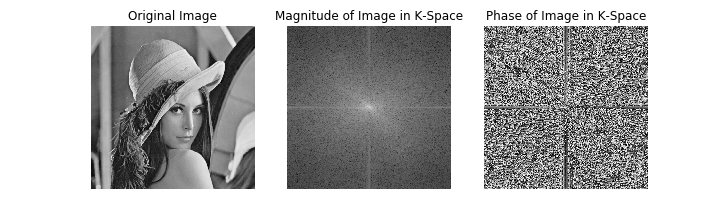
\includegraphics[width=.9\textwidth]{5/fft_example.png}
\caption{An example of the magnitude and phase of an image in k-space.}
\label{ch5:fft_example}
\end{figure}

The next step in our pipeline is to add scanner noise to the brain signal sequence. In a regular rs-fMRI of a patient, the noise in the sequence is the result of two factors: the spin history effects of motion and the susceptibility effects of motion. To simplify the simulation, we choose to model the resulting noise rather than the individual sources.

Signal acquired by MRI scanners is first recorded as a raw data matrix in k-space. K-space contains spatial frequency information. The coordinate system of k-space differs from the coordinate system of physical space. In k-space, the closer a point is to the center of a zero-centered data matrix, the lower its frequency or phase. The brighter a point in the raw data matrix is, the larger its magnitude. An example of the magnitude and phase of an image in k-space can be seen in Figure \ref{ch5:fft_example}.

Generally speaking, images contain more low-frequency information than high-frequency information. We wish to be able to control the amount of noise added to the magnitude and phase components independently, so we choose to add noise to the sequence in k-space.

When adding scanner noise to the brain signal sequence, we add noise to each image volume independently. The image volume is transformed from physical space into k-space using the fast Fourier transform (FFT). To force the image to be zero-centered, we perform an FFT shift on the Fourier space data. A matrix the same size and shape as the image volume is created. The matrix is then filled with complex Gaussian noise, $n(\vec{l})$ where

\begin{equation}
|n(\vec{l})| = w_m * r_m, r_m~N(0,1)
\end{equation}

\noindent and

\begin{equation}
\angle n(\vec{l}) = w_p * r_p, r_p~N(0,1)
\end{equation}

\noindent In these two equations, $\vec{l}$ is the location of the point in the matrix, $w_*$ represents the weight assigned to the component, $r_*$ represents the random noise variable independently generated from a standard normal distribution, and the subscripts $m$ and $p$ refer to the magnitude and phase components, respectively. The complex noise is weighted so that the magnitude of the noise has a greater contribution than the phase of the noise, that is $w_m > w_p$ 

The matrix of complex noise is added to the zero-centered k-space image volume. The noisy k-space volume is unshifted and undergoes an inverse Fourier transform to change the data back to physical space. This sequence containing both brain signal and scanner noise is referred to as the noisy sequence.

\subsubsection{Patient Movement}

Now that the ground truth brain orientation and BOLD signal have been established, patient motion can be added to the BOLD phantom sequence. One of the aims of this document is to establish that patients from different populations exhibit different motion patterns. As we have not yet established what those motion patterns are, we developed a generic motion model for the simulation.

During an rs-fMRI scan, a patient theoretically has the freedom to rotate his head around three different axes, translate his head along three different axes, or some combination of translations and rotations. Realistically, once a patient has settled in the scanner, it becomes difficult for his head to only undergo translation. It is more likely that he will rotate his head. For the simplicity of the simulation, we assume no head translations occur during the scan.

A rotational transformation can be represented as a matrix. Rotations about a single axis are represented as followed:

\begin{equation}
R_x(\alpha) = \begin{bmatrix}
 1 &  0          & 0     \\ 
 0 &  cos\alpha  & sin\alpha \\ 
 0 &  -sin\alpha & cos\alpha \\ 
\end{bmatrix}
\end{equation}
\begin{equation}
R_y(\beta) = \begin{bmatrix}
 cos\beta &  0 & -sin\beta \\ 
 0        &  1 & 0         \\ 
 sin\beta &  0 & cos\beta  \\ 
\end{bmatrix}
\end{equation}
\begin{equation}
R_z(\gamma) = \begin{bmatrix}
 cos\gamma  & sin\gamma  & 0 \\ 
 -sin\gamma & cos\gamma  & 0 \\ 
 0          & 0          & 1 \\ 
\end{bmatrix}
\end{equation}

Rotational transforms are applied to the origin of the image. However, the origin of the image is not necessary anatomically significant. Head motion naturally occurs about the base of the neck. We can approximate the location of the base of the neck by calculating the center of mass of the brain. First, the image volume is thresholded to separate the brain from the background. Then the locations of the ``on'' voxels are averaged to calculate the center of mass. 

Motion is added to the noisy image sequence one volume at a time. No motion is applied to the first volume in the sequence, but volume is used to calculate the center of mass of the brain. For each subsequent volume, the angles of rotation about the x-, y-, and z-axes are each randomly generated from a standard normal distribution to create rotational change matrices, $R_{*,\Delta}$ (where the subscript $*$ represents $x$, $y$, or $z$). The new rotations $R_{*,\Delta}$ are added to the rotations from the previous step $R_{*,i-1}$ to create the rotation matrices for the current volume, $R_{*,i}$:

\begin{equation}
R_{*,i} = R_{*,i-1} + R_{*,\Delta}
\end{equation}

The three rotational transformations are combined into one matrix via multiplication: 

\begin{equation}
R_i = R_{x, i}(\alpha) R_{y,i}(\beta) R_{z,i}(\gamma)
\end{equation}

The compound transformation $R_i$ is then applied to the image at the center of mass calculated from the original image volume. \textit{Note: Since the simulation is constrained by the assumption of no head translations, the center of mass will remain consistent throughout the image sequence.}

After the motion has been added to every image volume in the sequence, the final sequence (labeled Pseudo-BOLD Sequence in Figure \ref{ch5:spectr_flow}) is ready to be used in motion correction analyses.

\subsection{Implementation}

SPECTr is implemented in Python (version 3.7.3). The \lstinline{nipy} library (version 0.4.1) was used to load images, save images, and combine the functional ROIs. The \lstinline{numpy} library (version 1.17.4) was used for matrix manipulations involved in the brain signal and noise generation steps. The image processing library \lstinline{skimage} (version 0.14.2) was used to calculate the center of mass. The Python wrapper \lstinline{SimpleITK} (version 1.2.4) of the Insight Toolkit library for image analysis was used to perform the rotational transformations associated with patient motion.

The SPECTr source code is available on Github: \url{https://github.com/jmschabdach/SPECTr}.

\subsection{Simulated Sequences Experiments}

We generated 90 image sequences from the MNI152 proton density image and the default mode network functional ROIs using the process described in the previous section. The image sequences were divided into three groups with different degrees of scanner noise. All simulated images underwent both registration techniques described in Chapter \ref{ch:moco}. The registered images also underwent independent component analysis (ICA) using FSL's MELODIC (Multivariate Exploratory Linear Optimized Decomposition into Independent Components) tool.

The registered images underwent the same type of analysis as the clinical images. The ICA technique was used to determine how much brain signal was recovered by each registration technique.

This particular experiment is one of the first to investigate how much true BOLD signal is preserved through motion correction. One of the major drawbacks to existing motion correction pipelines is that they remove signals of interest along with noise. In clinical data, there is no way to know the ground truth signal contained within the image; however, simulated phantom images have a \textit{de facto} known ground truth signal. The design for this experiment can be used to evaluate how much BOLD signal is recovered by other motion correction pipelines, and how close the recovered signal is to the signal of interest.


\section{Clinical Cohorts}

Our clinical cohorts are composed of healthy subjects and subjects who have congenital heart disease (CHD).
The phrases congenital heart defects and congenital heart disease (CHD) both refer to defects in the heart or the vessels around the heart. These defects affect how blood moves into, through, and away from the heart. 
CHD has a worldwide prevalence of about 8 per 1000 live births, meaning about 1.35 million children are born with CHD every year. Many CHD patients are also affected by comorbidities, including neurodevelopmental disorders. Since the survivability of CHD has increased from 10\% to 90\%, the medical community is faced with a growing, aging population of CHD patients with a variety of neurological needs. Subjects in CHD studies provide a diverse set of data, particularly when it comes to studying motion in rs-fMRIs.

In this section, we provide a general overview of the impact of CHD on a global scale, the process for diagnosis, and additional risks associated with CHD. We then discuss the process of diagnosing neurodevelopmental comorbidities occurring with CHD and the impact of improved medical care on the CHD population. We end this section with a description of the three populations from which we obtained clinical rs-fMRI sequences.


\subsection{CHD Background}

CHD consists of a variety of defects that can affect any combination of the vessels and chambers of the heart with varying degrees of severity. The defects prevent the cardiopulmonary system as a whole from functioning correctly, but pinpointing and effectively treating the defects can be a complex process. It is important to note that each defect type has a different prevalence, a different treatment plan, and different expected outcomes. A breakdown of prevalence rates of some of the most common lesion types can be seen in Figure \ref{ch5:fig:usa-defects-prev}. 

Different presentations of CHD are associated with a number of different genetic and environmental factors \cite{Mozaffarian2016}. Genetic conditions such as Down syndrome, Turner syndrome, 22q11 deletion syndrome, Williams syndrome, and Noonan syndrome are associated with certain CHD presentations. Maternal behaviors such as smoking and binge drinking are known to cause heart problems in the fetus. Other maternal risk factors are obesity, folate deficiency, and living at a high altitude. Paternal exposure to phthalates, anesthesia, sympathomimetic medications, pesticides, and solvents may increase the risk of the fetus for developing CHD. While there are quite a few factors in this list, there are many CHD cases whose causes are unknown.

\begin{figure}
\centering
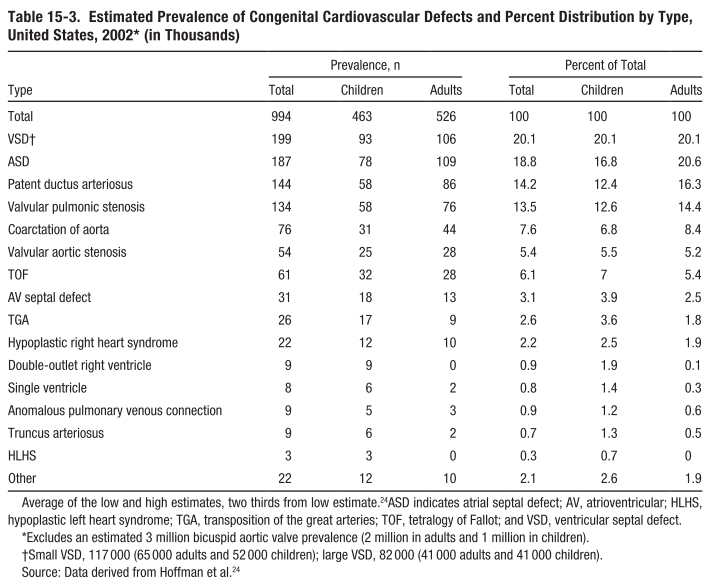
\includegraphics[width=0.6\textwidth]{5/chd-defects-usa.png}
\caption{Table of prevalences of congenital heart defects as compiled by \cite{Mozaffarian2016}.}
\label{ch5:fig:usa-defects-prev}
\end{figure}

Once a patient is diagnosed with one of these defects or a cause of the CHD is identified, the specific nature of his case must be clearly documented. The documentation of CHD using the International Classification of Diseases, Ninth Revision, Clinical Modification (ICD-9-CM) has 25 high-level codes representing various presentations of CHD, but these codes used alone are often not sufficient for describing a patient's true condition \cite{Mozaffarian2016}. Additional ICD-9-CM codes should be used to communicate the finer details of a patient's condition if they are available. 

The incidence of CHD in live births vary across countries and continents. The United States reports approximately 4-10 CHD cases per 1000 live births. Europe and Asia see about 6.9 and 9.3 CHD cases per 1000 live births, though smaller studies have been conducted in many countries to measure local prevalence \cite{Mozaffarian2016}. In China, the incidence of CHD ranges from 8.98 to 11.1 per 1000 live births \cite{Zhao2019} \cite{Qu2016}. 
A pair of studies from Iran report incidences of 8.6 and 12.3 per 1000 live births, though the studies note that they were performed in different geographical locations with different populations within the country \cite{Nikyar2011} \cite{Rahim2008}.
One report from Dharan reports an incidence of 5.8 per 1000 patients admitted to a tertiary care hospital over a 12 month period \cite{Shah2008}. A study of newborns at one hospital in New Delhi, India, claims an incidence of 3.9 per 1000 live births, though this rate may be a poor estimate as there is a significant delay between patient birth and referral to a cardiac center in India \cite{Khalil1994} \cite{Saxena2005}.

These incidence rates should be analyzed with some caution. In many cases, the reported rates were based on medical records. Medical records are not always correct; it is well known that human error can lead to a medical record lacking information or containing incorrect information. The only way for a person to have a medical record is for him or her to go to a medical center. Not everyone who has CHD is able to seek medical help, often because of their geographical locations or their income. Even if a patient is able to seek medical help, the availability of proper cardiac care varies between and within countries. However, it is generally expected that CHD incidence rates will increase as screening tools and treatments become more effective and more widespread, leading to earlier detection of defects.
 
% Diagnosis
Currently, the process of detecting and diagnosing CHD can begin before birth. A specialized ultrasound test called fetal echocardiography can detect heart abnormalities as early as the second trimester of the pregnancy. People who learn they are pregnant with a fetus who shows signs of CHD may choose to handle this information by opting for termination or pursuing a more detailed diagnosis. Additional tests such as amniocentesis and follow-up ultrasounds may be used to determine treatment options before the patient is born. Generally, severe CHD cases present and are detected at earlier stages of life, but minor defects may not become apparent until the patient is older. Tests used to diagnose CHD in postnatal patients include electro- and echo-cardiograms, chest x-rays, pulse oximetry, exercise stress tests, computed tomography or MRI scans, and cardiac catheterization. Treatment of different defects varies from monitoring and medication to surgery and cardiac implants.

\begin{figure}
\centering
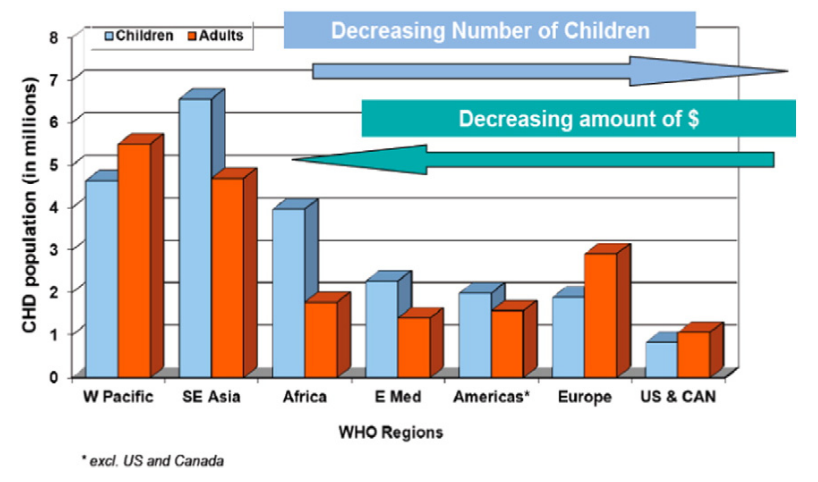
\includegraphics[width=0.7\textwidth]{5/CHD-burden-webb.png}
\caption{Estimated CHD burden in World Health Organization (WHO) regions using incidence rates of approximately 12/1000 and 4/1000 in children and adults, respectively \cite{Webb2015}.}
\label{ch5:fig:CHD-burden}
\end{figure}

%Depending on the cause of the 
The cost of diagnostic techniques and treatment plans impose different levels of the financial burden on CHD patients and their families. Certain defects require complex, expensive surgical repairs, while others can be treated with less expensive approaches \cite{Mozaffarian2016}. The burden of CHD across the globe was outlined by Webb et al. \cite{Webb2015}. Their figure illustrating the prevalence of CHD and the availability of funds with which to treat it can be seen in Figure \ref{ch5:fig:CHD-burden}. As the overall mortality of CHD declines, the burden of CHD is expected to increase \cite{Mozaffarian2016}.

% Complications and risks
Unfortunately, the cost of treating CHD is not the only burden a patient must undergo. Patients with CHD are also at increased risk for heart failure and infections \cite{Mozaffarian2016}. Children with CHD are at a 19-fold risk for stroke compared to their healthy counterparts \cite{Fox2015}. In a study of Swedish citizens born between 1970 and 1993, Giang et al. compared the prevalence of cardiac conditions in patients with and without CHD \cite{Giang2018}. They found that patients who had a CHD diagnosis were at about eight times higher risk for intracerebral hemorrhage and subarachnoid hemorrhage than their non-CHD counterparts. The CHD patients were also more likely to suffer from arrhythmia and heart failure. 

% When are patients diagnosed?
% Expected lifespan
% Treatment plan
% Financial burden

However, cardiac conditions are not the only complications CHD must deal with. Many of these patients also suffer from neurocognitive disorders that co-occur with CHD. Early research in this area focuses on the neurodevelopmental status of neonatal patients pre- and post-surgical intervention. One theory was that some factor or factors in the surgical intervention caused brain injuries in the patients. This idea proved to be inaccurate when researchers began detecting neurological malformations \textit{in utero}.

In a systematic review of available literature regarding prenatal and postnatal presurgical CHD cases and neurodevelopmental outcomes, Mebius et al. identify two theories about the causality of neurodevelopmental delays and CHD \cite{Mebius2017}. The first theory is that abnormalities in the cardiac system prevent the developing brain from receiving enough oxygen and nutrients, which disrupts prenatal brain development. The second theory is that faulty genetic pathways used during both cardiac and brain development cause both conditions to co-occur. However, 11 of the articles Mebius et al. found during their review suggest a third theory related to blood flow through the umbilical artery. During the prenatal period, a fetus receives oxygen from the mother via the placenta. If the placenta was not functioning correctly, it could lead to the fetus receiving not enough oxygen. Lower quantities of oxygen throughout prenatal development could potentially cause problems both in neurological and cardiac growth. The 11 articles have contradictory results, but some researchers are currently investigating the role of the placenta in CHD and prenatal brain development.

The survival of CHD patients to adulthood has increased from 10\% to 90\% over the last several decades as CHD diagnostic tools and treatments have improved.  Currently, Webb et al. estimate that at least 12 to 34 million adults have CHD, and this number is expected to increase \cite{Webb2015}. The impact of the combination of CHD and neurological conditions throughout a patient's lifetime is starting to be explored. The aging of the CHD population has also sparked interest in the relationships between CHD and adult-stage neurological disorders such as dementia and Alzheimer's. 

While the purpose of this study is not to focus on CHD patients, we chose to use CHD and aging brain images in support of research being performed in the area of relationships between CHD and neurodevelopment.

\subsection{Study Cohorts}

The rs-fMRIs used in this study were gathered as part of ongoing studies of the relationship between CHD and neurodevelopment. Data from the CHD/neurodevelopment studies was obtained through studies approved by the IRB at the Children's Hospital of Pittsburgh of UPMC and the University of Pittsburgh. All data are stored and accessed in compliance with HIPAA policies.

The subjects included in this analysis fall into three age groups: neonatal, preadolescent, and fetal. To summarize the cohorts, there were 124 neurological rs-fMRIs obtained for the fetal cohort, 163 neurological rs-fMRIs obtained for the neonatal cohort, and 546 neurological rs-fMRIs obtained for the preadolescent cohort. The fetal cohort also contains 105 rs-fMRIs of the placenta. The race, ethnicity, and gender counts for these three cohorts can be seen in Figures \ref{ch5:clinical:race}, \ref{ch5:clinical:eth}, and \ref{ch5:clinical:gender}, respectively. The majority of subjects in each cohort were white and male. In the following sections, we describe each cohort in detail. 

\begin{figure}
\centering
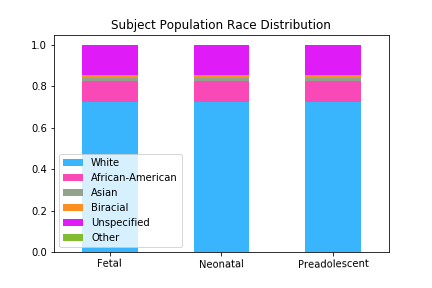
\includegraphics[width=.75\textwidth]{5/demo_clinical_subj_race.png}
\caption{Distribution of subject races for all three cohorts.}
\label{ch5:clinical:race}
\end{figure}%
%
\begin{figure}
\centering
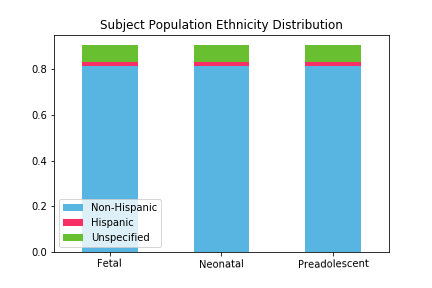
\includegraphics[width=.75\textwidth]{5/demo_clinical_subj_ethnicity.png}
\caption{Distribution of subject ethnicities for all three cohorts.}
\label{ch5:clinical:eth}
\end{figure}

\begin{figure}
\centering
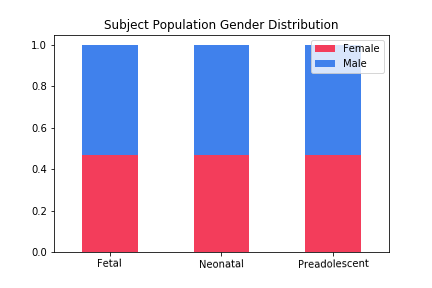
\includegraphics[width=.75\textwidth]{5/demo_clinical_subj_gender.png}
\caption{Distribution of subject genders for all three cohorts.}
\label{ch5:clinical:gender}
\end{figure}

\subsubsection{Fetal Subject Population and Images}


A fetal subject is scanned in vivo. He is suspended in amniotic fluid within his mother. The amniotic fluid has a buoyancy that reduces the effects of gravity and allows a fetal subject significant freedom of movement. The fetus can rotate, shift, and flip in ways that can only be accomplished when floating in a body of water. The properties of the uterus constrain the physical space in which motion could occur, but not as much as the head coil and gravity do to the other patient cohorts. A fetus is not guaranteed to be in any specific position at the start of the scan: the scan begins when the mother is ready, not when the fetus achieves a certain pose. 

The fetal subjects underwent fetal echocardiography scans in a cardiac clinic to determine whether they were healthy or had a form of CHD. Images of the fetal brain and the placenta were obtained for each subject during MRI acquisitions.

The MRI scans are performed when the mother is in her third trimester. Due to the constraints of pregnancy, the mother cannot lay directly on her side or directly on her back. The MRI scans were performed with the mother going feet first into the scanner and laying on an angle on her left or right side (left or right anterior oblique). The side chosen is the mother's preference. Her back is supported by a pillow to maintain her position during the scan. A large flexible coil is positioned on her abdomen to get coverage of the fetus and the placenta. The coil and pillow are secured with a strap. The mother is fitted with earplugs and headphones and given a button to use during the scan if she needs to get the attention of the radiology technician. No vital monitoring occurs as part of the study.

\begin{figure}
\centering
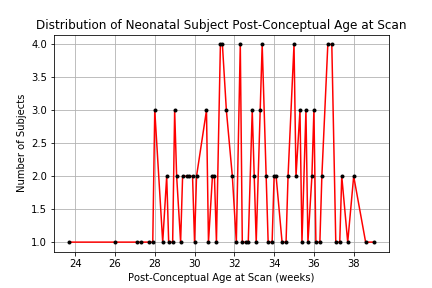
\includegraphics[width=.75\textwidth]{5/demo_fetal_scan_pca.png}
\caption{The distribution of post-conceptual ages at the time of the scan of all fetal subjects.}
\label{ch5:fetal:scanpca}
\end{figure}

\begin{figure}
\centering
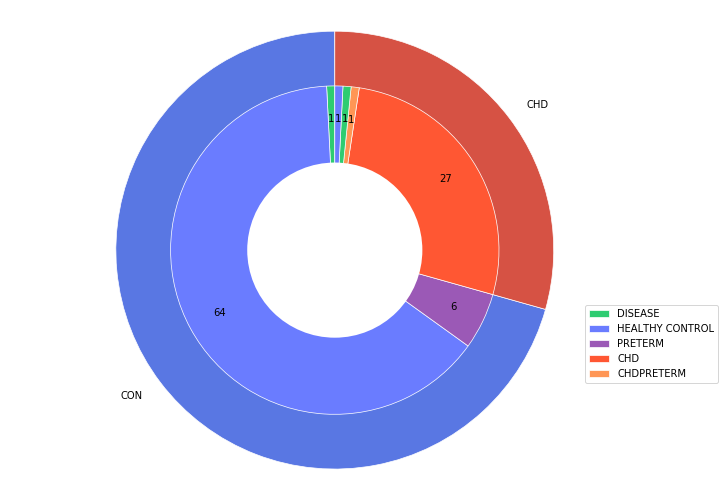
\includegraphics[width=.9\textwidth]{5/demo_fetal_subj_cohort.png}
\caption{The outer ring represents the group the subject was assigned to based on the fetal examination while the inner ring represents the group the subject was assigned to after birth.}
\label{ch5:fetal:cohort}
\end{figure}

A total of 124 fetal subjects were scanned on a 3T Skyra (Siemens AG, Erlangen, Germany). The subjects were between 23 and 39 weeks old post-conception. The distribution of fetal post-conceptual age at the time of the scan can be seen in Figure \ref{ch5:fetal:scanpca}. Axial rs-fMRI brain scans were acquired for all subjects and placental rs-fMRI scans were acquired for 105 subjects. The subjects were divided into CHD and control groups based on fetal examinations. Some subjects were moved to different groups after birth. A breakdown of these groups before and after birth can be seen in Figure \ref{ch5:fetal:cohort}.

The parameters for the fetal rs-fMRI protocol were FOV = 300 mm and TE/TR = 32/2280 ms with an interplane resolution of 4.7 x 4.7 mm, slice thickness of 3.0 mm and no gap between slices. The sequences were 150 volumes in length, and each volume was composed of 32 slices containing 64 x 64 voxels. Each brain or placenta image underwent manual segmentation by one of a group of four researchers to remove non-brain or non-placental tissues, respectively, from the image. 


%Real goal is to develop a method of registering the fetal brain and placental images so that we can further examine the relationship between placental oxygen levels and fetal brain development. Longitudinally, this technique can be used to determine how placental oxygen flow and fetal brain development impact a patient over the course of his or her life. Once the relationship between the placenta and fetal brain development is better understood, we can determine a set of neuroprotective interventions to employ for at-risk patients before they are born.

We are interested in both the fetal brain and placental images for our work partially because of the relationship between placenta and brain development, but also because these organs have very different physical properties. The fetal brain is a rigid structure floating and moving within the amniotic fluid. It undergoes translation and rotation as a single unit due to passive and active maternal and fetal motions. The placenta, on the other hand, is anchored in place on the uterine wall. It may undergo small translations or rotations due to maternal motion, but it will respond differently to fetal motion. Fetal motions cause nonlinear deformations of the pliable placenta that can only be adequately accounted for using nonlinear registration algorithms. Nonlinear registrations have the potential to deform brain images into physically impossible shapes, so the fetal brain and placenta were manually segmented in their respective images so that each organ could undergo independent motion correction. As the fetal subjects have both brain and placenta images, their data will be used to examine the impact of volume registration on different organ types.

%ELEPHANTS DISCUSSION?
%Fetal subjects have different constraints on their physical environment than neonates, preadolescents, and adults. As a result, they exhibit unique patterns of motion. The previous subject cohorts discussed in this chapter have the following commonalities: the subject experiences the full effects of gravity, the subject is lying on his back in an MRI scanner, and the subject's head motion is limited by the head coil within the MRI. Any motion in these images is a direct result of the subject himself moving, whether passively (cardiac motion and breathing) or actively (fidgeting or looking around).

\subsubsection{Neonatal Subject Population and Images}

Neonatal subjects have been recruited as part of a prospective observational study. This cohort was scanned at two sites. At Site 1, the subjects were scanned using either a 3T Skyra (Siemens AG, Erlangen, Germany) or a 3T Signa (GE Healthcare, Chicago, Illinois, United States of America). At Site 2, the subjects were scanned using a 3T Achieva (Koninklijke Philips N.V., Amsterdam, Netherlands).

The subjects were unsedated during the scans, and a ``feed and bundle'' protocol was used to prevent movement \cite{Windram2011}. The newborns were positioned in the coil to minimize head tilting. Newborns were fitted with earplugs (Quiet Earplugs; Sperian Hearing Protection, San Diego, CA) and neonatal ear muffs (MiniMuffs; Natus, San Carlos, CA). An MR-compatible vital signs monitoring system (Veris, MEDRAD, Inc. Indianola, PA) was used to monitor neonatal vital signs. All scans were performed using a multi-channel head coil. The parameters for the resting-state BOLD MR scans were FOV=240 mm and TE/TR=32/2020 ms with an interplane resolution of 4x4 mm, slice thickness of 4 mm, and 4 mm space between slices. The acquired images contained 150 volumes where each volume consisted of 64x64x32 voxels$^3$.

\begin{figure}
\centering
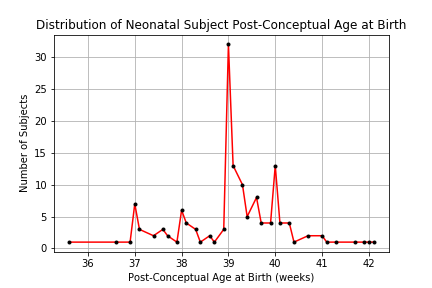
\includegraphics[width=.75\textwidth]{5/demo_neonate_subj_pca.png}
\caption{The distribution of post-conceptual ages at birth of all neonatal subjects.}
\label{ch5:neonates:birthpca}
\end{figure}

\begin{figure}
\centering
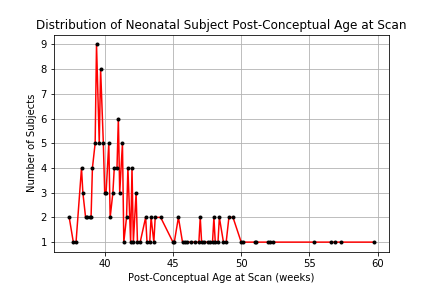
\includegraphics[width=.75\textwidth]{5/demo_neonate_scan_pca.png}
\caption{The distribution of post-conceptual ages at the time of the scan of all neonatal subjects.}
\label{ch5:neonates:scanpca}
\end{figure}

Scans from a total of 149 patients were included in this work. The average post-conceptual age of the patients at birth was 39.08 weeks, and they were on average 42.64 weeks post-conception at the time of the scan. The distribution of post-conceptual ages of the subjects at birth and at the time of the scan can be seen in Figure \ref{ch5:neonates:birthpca} and Figure \ref{ch5:neonates:scanpca}. 

\begin{figure}
\centering
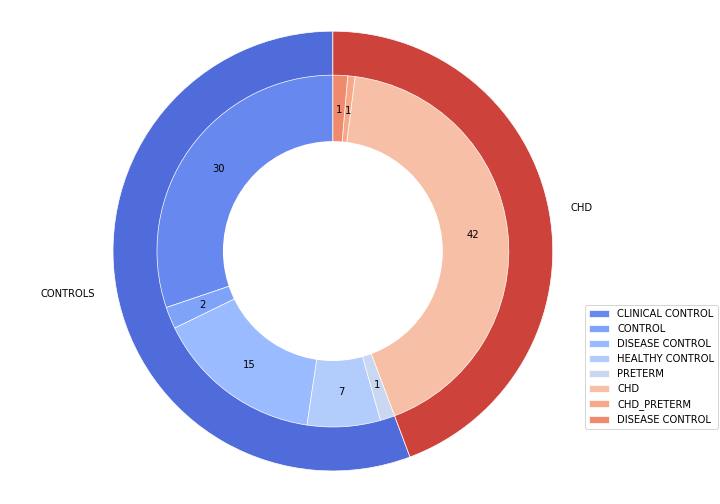
\includegraphics[width=.75\textwidth]{5/demo_neonate_subj_cohort.png}
\caption{The breakdown of subject groups contained in the Control and CHD neonatal cohorts.}
\label{ch5:neonates:cohorts}
\end{figure}

The subjects were a mix of control subjects and CHD subjects. A comprehensive breakdown description of the subgroups within these two cohorts can be seen in Figure \ref{ch5:neonates:cohorts}. In this figure, the term ``Control'' encompasses both healthy full-term subjects, healthy pre-term subjects, and non-CHD clinical subjects (clinical control and disease control). The CHD group is composed of subjects diagnosed with CHD who were either born full-term or pre-term. Of the entire cohort, 14 subjects underwent two scanning sessions resulting in 163 rs-fMRI scans.

% ELEPHANTS DISCUSSION?
As the neonates were most often asleep during the scan, they exhibit less motion overall compared to our other clinical cohorts. The high-motion neonates are an obvious exception to this concept, but many of the high-motion images contained long periods where the subject was stationary. Applying both the DAG-based framework and the traditional registration framework to these images provided the opportunity to compare the performances of both registration frameworks to each other in the context of the usability gold standard thresholds. 

\subsubsection{Preadolescent Subject Population and Images}

\begin{figure}
\centering
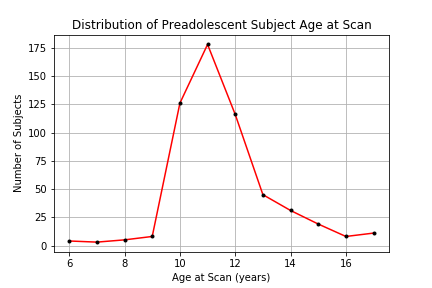
\includegraphics[width=0.5\textwidth]{5/demo_pread_scan_age.png}
\caption{The distribution of preadolescent subject ages at the time of the scan.}
\label{fig:pread_sites}
\end{figure}

\begin{figure}
\centering
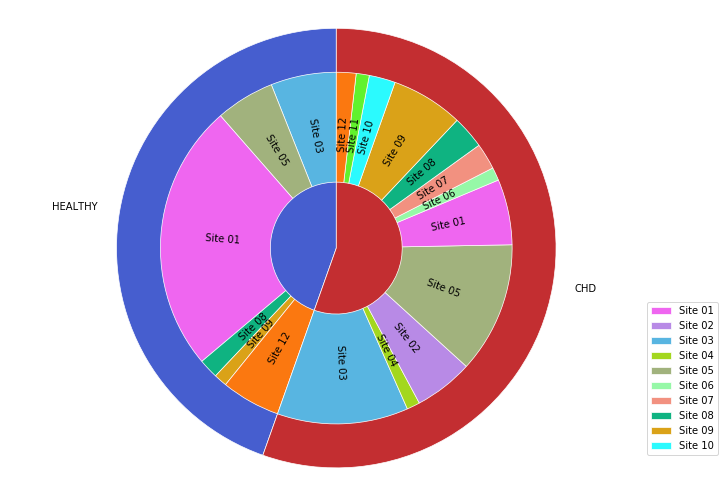
\includegraphics[width=0.5\textwidth]{5/demo_pread_subj_cohort.png}
\caption{The distribution of CHD and healthy subjects between the 12 sites enrolled in the preadolescent study.}
\label{fig:pread_ages}
\end{figure}

\begin{table}[]
\centering
\caption{The number of CHD and healthy control preadolescent subjects scanned on each scanner type at each site.}
\label{tab:pread-site-counts}
\begin{tabular}{|c|c|c|c|c|}
\hline
\textbf{Site} & \textbf{Scanner} & \textbf{Field Strength} & \textbf{CHD} & \textbf{HEALTHY} \\ \hline
Site 01 & Skyra   & 3T & 22.0 & 128.0 \\ \hline
Site 02 & Unknown & Unknown & 24.0 & 0.0   \\ \hline
Site 03 & Skyra   & 3T & 83.0 & 44.0  \\ \hline
Site 04 & Unknown & Unknown  & 8.0  & 0.0   \\ \hline
Site 05 & Prisma  & 3T & 23.0 & 12.0  \\ \hline
Site 05 & Skyra   & 3T & 50.0 & 26.0  \\ \hline
Site 06 & Prisma  & 3T & 6.0  & 0.0   \\ \hline
Site 07 & Trio    & 3T & 14.0 & 0.0   \\ \hline
Site 08 & Prisma  & 3T & 15.0 & 13.0  \\ \hline
Site 09 & Ingenia & 3T & 23.0 & 4.0   \\ \hline
Site 10 & Prisma  & 3T & 14.0 & 0.0   \\ \hline
Site 11 & Skyra   & 3T & 4.0  & 0.0   \\ \hline
Site 12 & Skyra   & 3T & 11.0 & 32.0  \\ \hline
\end{tabular}
\end{table}

As part of a multicenter study of CHD in preadolescents, rs-fMRIs have been collected from twelve sites throughout the United States. The two sites from the neonatal study in the previous section also participated in this study and retained their respective labels. The subjects enrolled in this study were patients in the age range of 6 to 17 years (average age: 11 years) who either had CHD or were healthy with no neurocognitive impairments. The histogram of patient ages at the time of each scan can be seen in Figure \ref{fig:pread_ages}.

The majority of the subjects have CHD, though six sites also recruited healthy patients. The distribution of CHD and healthy subjects between the 12 sites can be seen in Figure \ref{fig:pread_sites} and in more detail in Table \ref{tab:pread-site-counts}.

The subjects underwent neurodevelopmental testing prior to the neurological MRI scans. The neurodevelopmental testing was scheduled to take between 4.5 and 5 hours. The subject is given breaks to reduce study fatigue. The MRI scans were scheduled to take 60 minutes, assuming approximately 50 minutes of actual scan time and no repeat acquisitions. 

As discussed earlier in this document, patient preparation and education before a scan can help reduce the amount of motion in the scan. The process used at Site 1 is partially dependent on the age of the preadolescent subjects. For younger subjects under the age of 8 years old, both the subject and the subject's family are asked whether they believe the subject could remain still for 45 minutes. The subject may also be shown the scanner to help determine his response. If the subject is comfortable being still for 45 minutes, the subject will undergo training with a mock scanner and the scan will be scheduled. For subjects older than 8 years, the subject himself determines whether or not he will undergo a brain scan. He also determines if he would like to undergo training with the mock scanner prior to the scan. This process or similar processes may be used at the other sites in the study.

During the scan itself, the subject is provided with ear protection in the form of earplugs and headphones. A stereotactic marker (vitamin capsule) is taped to the subject's right temple. The patient's head is positioned in a head coil so that his head and neck muscles are relaxed but not causing any head rotation. For comfort and lower body stabilization, his back or legs may be supported with an MR compatible pillow or foam pad. Additional pads or sponges may be used to stabilize and support the head. All subjects are positioned to that the centering crosshairs in the head coil are located at the subject's nasion (between the eyebrows). The patient is given a squeeze ball alarm to use if he becomes distressed during the scan and is reminded to remain still during the scan. 

At Site 1, the research coordinator performs verbal checks on the subjects between every or every other scanning protocol during the same acquisition period. During the rs-fMRI scan, a star is projected onto a screen outside the scanner. The screen is reflected in the subject's line of sight via a mirror attached to the head coil. The subject is instructed to focus on the star during the rs-fMRI scan.

The parameters for the rs-fMRI scans were FOV = 256 mm and TE/TR = 32/650 ms with an interplane resolution of 4.0 x 4.0 mm, slice thickness of 4.0 mm and no gap between slices. At the sites using Siemens scanners, the sequences were 470 volumes in length while the sites using Philips scanners had sequences with a length of 380 volumes. Each volume was composed of 36 slices containing 64 x 64 voxels.

The multicenter imaging study of preadolescent subjects provides a unique opportunity to evaluate the efficacy of the DAG-based framework on a large subject cohort containing variable amounts of motion. %The outcome of this experiment will be used in the next experiment to determine if there are any site-specific or vendor-specific variables influencing patient motion.

\section{Summary}

In this chapter, we discussed our two major data sets, a simulated data set and a clinical data set. 

The simulated data were generated using an rs-fMRI simulation pipeline developed in-house and were used for the purpose of measuring ground truth signal recovered by motion correction techniques. A structural image from the ICBM Average Brain project and a set of functional ROIs associated with resting-state networks were used to generate the data. The data was given simulated scanner noise in the form of Gaussian noise injected into the k-space of the image. Finally, each image underwent rotation about the center of mass of the brain.

The pediatric data were obtained through prospective studies of CHD and neurodevelopment being conducted at the UPMC Children's Hospital of Pittsburgh. CHD is a complex disease affecting millions of people globally. As the new treatments for CHD and its comorbidities have evolved, the life expectancy of patients with CHD has also increased. 

Some of the comorbidities of CHD are related to a patient's neurological development. As part of three studies of the relationship between CHD and brain development, rs-fMRI sequences of fetal, neonatal, and preadolescent brains have been gathered. A set of placental images was acquired alongside the fetal neurological images. The pediatric images were used to compare the two volume registration techniques on a diverse set of clinical data. We also used these images to examine patterns of motion unique to different age groups. 


In the next chapter, we examine the results of the registration methods and of the machine learning techniques applied to the motion metrics for the images.
